\documentclass[spanish, aspectratio=169]{beamer}

\usepackage[es-tabla]{babel}
\usepackage{parskip}
\usepackage[capitalise, noabbrev]{cleveref}
\crefname{table}{\spanishtablename}{\spanishtablename}



\title{
	\textbf{
		Desarrollo de un modelo fundacional estocástico basado en procesos Gaussianos para la clasificación de bioseñales EEG en el diagnóstico asistido del TDAH.
	}
	}
\author{
	Julián David Pastrana Cortés, M.Sc.
	}


\date{}

\begin{document}
	
	
\frame{\titlepage}

\begin{frame}{Motivation}
	\begin{block}{}
		Mental disorders affect cognition, behavior, and emotions of millions of people worldwide. Around 350 million individuals suffer from a mental disorder [1].
	\end{block}
	
	\begin{columns}
		\column{0.33\textwidth}
		\centering
		
\includegraphics[width=0.5\textwidth]{figures/OppositionalDefiantDisorder.png}
		
		\vspace{0.5em}
		\textbf{Oppositional Defiant Disorder}
		
		\column{0.33\textwidth}
		\centering
		
\includegraphics[width=0.5\textwidth]{figures/BipolarDisorder.png}
		
		\vspace{0.5em}
		\textbf{Bipolar Disorder}
		
		\column{0.33\textwidth}
		\centering
		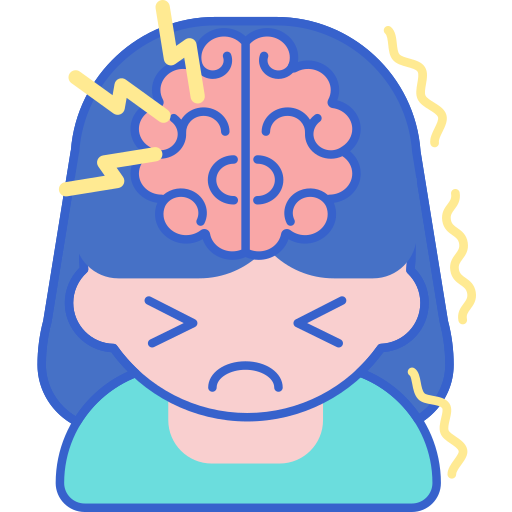
\includegraphics[width=0.5\textwidth]{figures/ADHD.png}
		
%		\vspace{0.5em}
		\textbf{Attention Deficit Hyperactivity Disorder}
	\end{columns}
	
	\pause
	\begin{block}{Challenges:}
		lengthy follow-up, subjective interpretations, inefficient criteria, and limited access to clinical care.
	\end{block}
	
\end{frame}

\begin{frame}{Problem Statement and Research Question}
	
\renewcommand{\arraystretch}{1.5} 

\begin{table}[htbp]
	\centering
	\footnotesize
	\begin{tabular}{>{\raggedright\arraybackslash}p{3.1cm} >{\centering\arraybackslash}p{2cm} >{\centering\arraybackslash}p{2cm} >{\centering\arraybackslash}p{2cm} >{\centering\arraybackslash}p{2cm}}
		\toprule
		\diagbox{\textbf{Model}}{\textbf{Challenge}} & \textbf{Complex Patterns} & \textbf{High Labeled Data Volume} & \textbf{Stochasticity} & \textbf{Data Shift} \\
		\midrule
		Traditional Machine Learning Models[2, 3] & \textcolor{purple}{\ding{55}} & \textcolor{purple}{\ding{55}} & \textcolor{teal}{\ding{51}} & \textcolor{purple}{\ding{55}} \\[1mm]
		Traditional Deep Learning Models [4, 5]    & \textcolor{teal}{\ding{51}}    & \textcolor{purple}{\ding{55}} & \textcolor{teal}{\ding{51}} & \textcolor{purple}{\ding{55}} \\[1mm]
		Foundation Models[6]                   & \textcolor{teal}{\ding{51}}    & \textcolor{teal}{\ding{51}}    & \textcolor{purple}{\ding{55}} & \textcolor{purple}{\ding{55}} \\
		\bottomrule
	\end{tabular}

\end{table}


	
	
\pause	
	
	
	\begin{block}{Research Question}
		\footnotesize
		How to develop a stochastic foundational model for inference from biological signals that integrates Gaussian processes to support clinical practice through EEG signal analysis, considering the variability and inconsistencies present in the datasets?
	\end{block}	
\end{frame}

\begin{frame}{Objectives}
	\vspace{-0.3cm}
	\begin{block}{General Objective}
		\small
		Develop a stochastic learning methodology related to EEG recordings based on a foundational model that integrates labeled and unlabeled databases using self-learning and fine-tuning techniques.
	\end{block}
	
	\vspace{-0.1cm}
	\begin{block}{Specific Objectives}
		\small
		\begin{enumerate}
			\item Develop a foundational model for the classification of biological signals related to EEG recordings, leveraging \textcolor{MyAccent}{unlabeled data} during the self-learning phase and labeled data for fine-tuning.
			\item Implement a \textcolor{MyAccent}{stochastic prediction} tool based on Gaussian processes to model uncertainty in the foundational model's predictions.
			\item Design a strategy to \textcolor{MyAccent}{manage variability and inconsistency} in EEG recording datasets, enabling the effective integration of databases with diverse standards.
		\end{enumerate}
	\end{block}
\end{frame}

\begin{frame}[fragile]{Foundation Model Workflow}
	\centering
	\resizebox{\textwidth}{!}{
		\begin{tikzpicture}[font=\sffamily, >=stealth, node distance=3cm, thick]
			
			% Left Square (Training)
			\node[rectangle, draw=MyAccent, fill=MyLightGray, rounded corners, align=left, text=MyDarkBlue] (training) {
				\textbf{Data}\\[5pt]
				- Text\\
				- Images\\
				- Sensors\\
				- Speech
			};
			
			% Foundation Model (center)
			\node[rectangle, draw=MyAccent, fill=MyAccent!20, rounded corners, minimum width=3.5cm, minimum height=2cm, right=of training, text=MyDarkBlue] (foundation) {
				\textbf{Foundation Model}
			};
			
			% Right Square (Tasks)
			\node[rectangle, draw=MyAccent, fill=MyLightGray, rounded corners, align=left, right=of foundation, text=MyDarkBlue] (tasks) {
				\textbf{Task}\\[5pt]
				- Object Recognition\\
				- Text Generation\\
				- Sentiment Analysis\\
				- Image Captioning
			};
			
			% Arrows
			\draw[->, MyDarkBlue] (training.east) -- node[above, text=MyDarkBlue]{Pre-Training} (foundation.west);
			\draw[->, MyDarkBlue] (foundation.east) -- node[above, text=MyDarkBlue]{Fine-Tuning} (tasks.west);
			
		\end{tikzpicture}
	}
\end{frame}


% Include this frame in your Beamer document
\begin{frame}{\textcolor{MyDarkBlue}{Point Estimation vs. Distribution Estimation}}
	\centering
	\begin{tikzpicture}
		\begin{groupplot}[
			group style={
				group name=my plots,
				group size=2 by 1,
				horizontal sep=1cm,
			},
			width=5cm,
			height=4cm,
			scale only axis,
			axis lines=left,
			ymin=0, ymax=1,
			xmin=0, xmax=5.5,
			xlabel style={text=MyDarkBlue},
			title style={text=MyDarkBlue},
			]
			% Left subplot: Point Estimate Prediction
			\nextgroupplot[
			title={Point Estimation},
			xticklabel=\empty,
			yticklabel=\empty,
			]
			\addplot+[smooth, thick, color=MyAccent!30, mark=*,
			mark options={fill=MyAccent, draw=MyAccent}
			] coordinates {(0,0.2) (1,0.3) (2,0.5) (3,0.7) (4,0.8)};
			\addplot[only marks, mark=*, MyDarkBlue] coordinates {(5,0.85)};
			
			% Right subplot: Distribution Estimation with Error Bars
			\nextgroupplot[
			title={Distribution Estimation},
			xticklabel=\empty,
			yticklabel=\empty,
			]
			\addplot+[smooth, thick, color=MyAccent!30, mark=*,
			mark options={fill=MyAccent, draw=MyAccent}
			] coordinates {(0,0.2) (1,0.3) (2,0.5) (3,0.7) (4,0.8)};
			
			% Predictive distribution at time=5
			\addplot[name path=right, domain=0.65:1.05, variable=\y, samples=100, draw=none]
			({5 + 0.2*exp(-((\y-0.85)^2)/(2*0.004))}, {\y});
			
			\addplot[name path=left, domain=0.65:1.05, variable=\y, samples=100, draw=none]
			({5 - 0.2*exp(-((\y-0.85)^2)/(2*0.004))}, {\y});
			
			\addplot[fill=MyAccent!50, fill opacity=0.4, draw=none]
			fill between[of=right and left];
			
			\addplot[only marks, mark=*, MyDarkBlue] coordinates {(5,0.85)};
			
		\end{groupplot}
	\end{tikzpicture}
	
	\begin{block}{}
		Sometimes, a single point prediction is not enough. How confident is the model in its prediction?
	\end{block}
\end{frame}


\begin{frame}[fragile]{Architecture}
	\resizebox{\textwidth}{!}{
		\tikzset{trapezium stretches=true}
		\centering
		\begin{tikzpicture}[font=\sffamily, >=stealth, node distance=8mm]
			% Latent variable (z)
			\node[rectangle, fill=MyAccent, text=white, font=\sffamily\large, minimum height=3cm, text width=3cm, align=center] (z) {Latent\\ Representation};
			
			% Encoder trapezoid
			\node[trapezium, fill=MyAccent!20, minimum width=4cm, minimum height=4cm,
			trapezium left angle=86, trapezium right angle=86, shape border rotate=270,
			anchor=east, left=5mm of z, font=\sffamily\large, text=MyDarkBlue] (enc) {Encoder};
			
			% Decoder trapezoid
			\node[trapezium, fill=MyAccent!20, minimum width=4cm, minimum height=4cm,
			trapezium left angle=86, trapezium right angle=86, shape border rotate=90,
			anchor=west, right=5mm of z, font=\sffamily\large, text=MyDarkBlue] (dec) {Decoder};
			
			% Gaussian Process circle
			\node[circle, fill=MyAccent!20, text=MyDarkBlue, font=\sffamily\small,
			below=2cm of z, minimum size=2cm, align=center] (gp) {Gaussian\\Process};
			
			% Arrows and labels
			\draw[->, MyDarkBlue, thick] (enc.west) -- ++(-1.5,0) node[left, align=right, text=MyDarkBlue] {Input};
			\draw[->, MyDarkBlue, thick] (dec.east) -- ++(1.5,0) node[right, align=left, text=MyDarkBlue] {Reconstruction};
			\draw[->, MyAccent, thick] (z.south) -- (gp.north);
			\draw[->, MyDarkBlue, thick] (gp.east) -- ++(1.5,0) node[right, align=left, text=MyDarkBlue] {Predictive Distribution\\(Inference)};
		\end{tikzpicture}
	}
\end{frame}


	
\end{document}
